\documentclass[a4paper]{article}
\usepackage[spanish]{babel}
\usepackage[utf8]{inputenc}
\usepackage{charter}   % tipografia
\usepackage{graphicx}
%\usepackage{makeidx}
\usepackage{paralist} %itemize inline
\usepackage{booktabs}

%\usepackage{float}
%\usepackage{amsmath, amsthm, amssymb}
%\usepackage{amsfonts}
%\usepackage{sectsty}
%\usepackage{charter}
%\usepackage{wrapfig}
%\usepackage{listings}
%\lstset{language=C}


\usepackage{color} % para snipets de codigo coloreados
\usepackage{fancybox}  % para el sbox de los snipets de codigo

\definecolor{litegrey}{gray}{0.94}

% \newenvironment{sidebar}{%
% 	\begin{Sbox}\begin{minipage}{.85\textwidth}}%
% 	{\end{minipage}\end{Sbox}%
% 		\begin{center}\setlength{\fboxsep}{6pt}%
% 		\shadowbox{\TheSbox}\end{center}}
% \newenvironment{warning}{%
% 	\begin{Sbox}\begin{minipage}{.85\textwidth}\sffamily\lite\small\RaggedRight}%
% 	{\end{minipage}\end{Sbox}%
% 		\begin{center}\setlength{\fboxsep}{6pt}%
% 		\colorbox{litegrey}{\TheSbox}\end{center}}

\newenvironment{codesnippet}{%
	\begin{Sbox}\begin{minipage}{\textwidth}\sffamily\small}%
	{\end{minipage}\end{Sbox}%
		\begin{center}%
		\vspace{-0.4cm}\colorbox{litegrey}{\TheSbox}\end{center}\vspace{0.3cm}}



\usepackage{fancyhdr}
\pagestyle{fancy}

%\renewcommand{\chaptermark}[1]{\markboth{#1}{}}
\renewcommand{\sectionmark}[1]{\markright{\thesection\ - #1}}

\fancyhf{}

\fancyhead[LO]{Sección \rightmark} % \thesection\ 
\fancyfoot[LO]{\small{Juli\'{a}n Palladino, Nicol\'{a}s De Carli, Mart\'{i}n Fosco}}
\fancyfoot[RO]{\thepage}
\renewcommand{\headrulewidth}{0.5pt}
\renewcommand{\footrulewidth}{0.5pt}
\setlength{\hoffset}{-0.8in}
\setlength{\textwidth}{16cm}
%\setlength{\hoffset}{-1.1cm}
%\setlength{\textwidth}{16cm}
\setlength{\headsep}{0.5cm}
\setlength{\textheight}{25cm}
\setlength{\voffset}{-0.7in}
\setlength{\headwidth}{\textwidth}
\setlength{\headheight}{13.1pt}

\renewcommand{\baselinestretch}{1.1}  % line spacing


% \setcounter{secnumdepth}{2}
\usepackage{underscore}
\usepackage{caratula}
\usepackage{url}


% ******************************************************** %
%              TEMPLATE DE INFORME ORGA2 v0.1              %
% ******************************************************** %
% ******************************************************** %
%                                                          %
% ALGUNOS PAQUETES REQUERIDOS (EN UBUNTU):                 %
% ========================================
%                                                          %
% texlive-latex-base                                       %
% texlive-latex-recommended                                %
% texlive-fonts-recommended                                %
% texlive-latex-extra?                                     %
% texlive-lang-spanish (en ubuntu 13.10)                   %
% ******************************************************** %



\begin{document}


\thispagestyle{empty}
\materia{Organización del Computador II}
\submateria{Segundo Cuatrimestre de 2014}
\titulo{Trabajo Práctico II}
\subtitulo{subtitulo del trabajo}
\integrante{Fosco, Martin Esteban}{449/13}{mfosco2005@yahoo.com.ar}
\integrante{Palladino, Juli\'{a}n}{231/13}{julianpalladino@hotmail.com}
\integrante{De Carli, Nicol\'{a}s}{164/13}{nikodecarli@gmail.com}

\maketitle
\newpage

\thispagestyle{empty}
\vfill
\begin{abstract}



\end{abstract}

\thispagestyle{empty}
\vspace{3cm}
\tableofcontents
\newpage


%\normalsize
\newpage

\section{Objetivos generales}

Este Trabajo Pr\'{a}ctico se ha centrado en explorar el modelo de programaci\'{o}n \textbf{SIMD}, us\'{a}ndolo para una aplicaci\'{o}n popular del set de instrucciones SIMD de intel (SSE), procesamiento de im\'{a}genes y videos.\\
En particular, se implementaron 4 filtros de im\'{a}genes: Cropflip, Sierpinski, Bandas y Motion Blur.\\


\section{Desarrollo}

\subsection{Explicaci\'{o}n de Implementaciones en assembler}

\subsubsection{Cropflip}
En el filtro Cropflip utilizamos aritm\'{e}tica de punteros para empezar a escribir en la \'{u}tima fila de la imagen destino mientras se lee de la primer fila de la parte a recortar de la imagen fuente. Al cambiar de fila, el puntero de escritura (\textit{rsi}) decrece, mientras que el de lectura crece (\textit{rdi}). A su vez, utilizamos 3 contadores: De Bytes horizontales (\textit{r11}), de Bytes verticales (\textit{EAX}) y \textit{r10} como backup de \textit{rbx}, para cuando es modificado. \'{E}ste \'{u}ltimo sirve. El SIMD es aprovechado al m\'{a}ximo, ya el movimiento es de a 4 p\'{i}xeles.

\subsubsection{Sierpinski}
El filtro Sierpisnki es procesado de la siguiente manera:

\begin{itemize}
\item Cargamos de la memoria 4 p\'{i}xeles, los desempaquetamos a dwords y luego los convertimos a floats, para poder calcular el \textit{coef}de cada uno. Quedan entonces en \textit{xmm0}, \textit{xmm1}, \textit{xmm2} y \textit{xmm3}, con sus componentes como floats.\\

\item Luego, para calcular el coef de cada p\'{i}xel, utilizamos valores ya cargados antes del ciclo (Por ejemplo \textit{255/cols} en \textit{xmm12} y \textit{255/filas} en \textit{xmm11}). \\

\item Se multiplica el coef por todos los componentes de cada pixel al mismo tiempo utilizando SIMD. \\

\item Por \'{u}ltimo se convierten y empaquetan estos 4 p\'{i}xeles a Bytes, guardados en \textit{xmm0}, y desde all\'{i} son almacenados al destino. 

\end{itemize}


\subsubsection{Bandas}

El filtro Bandas lo intentamos implementar tres veces. En esas tres fuimos variando la forma de pensar el filtro, sobretodo el 'branching' que generaba la parte de pasar de la suma de R, G y B al n\'{u}mero que ten\'{i}amos que guardar en el destino.\\
\begin{itemize}
\item Con condicionales: \\ \\
 La primer manera (la m\'{a}s ineficiente de las 3) fue intentar replicar el c\'{o}digo C y hacer los condicionales correspondientes. Esta forma no s\'{o}lo result\'{o} ser la m\'{a}s d\'{i}ficil de implementar (El c\'{o}digo se torn\'{o} muy largo y confuso), sino que nos dimos cuenta r\'{a}pidamente que era extremadamente ineficiente y no llegamos a terminarla. \\
\item Con c\'{a}lculos: \\ \\
 La segunda forma consisti\'{o} en aplicar una cuenta matem\'{a}tica para pasar de la suma (de R, G y B) al resultado final (La cuenta en s\'{i} era res=[([suma/96]+1)/2]*64 ). Esta nueva manera de pensar el ejercicio consigi\'{o} eliminar el enorme branching que generaban los condicionales de la implementaci\'{o}n anterior, pero todav\'{i}a podr\'{i}a ser optimizado a\'{u}n m\'{a}s.
\item Con m\'{a}scaras: \\ \\
Finalmente, por consejo de algunos docentes, decidimos implementar el ejercicio con el uso de m\'{a}scaras. La idea es, en cada iteraci\'{o}n: \\
\begin{itemize}
\item Levantar cuatro p\'{i}xeles en un XMM.\\
\item Luego en otros dos XMM hacer rotaciones para que queden alineados verticalmente los R, G y B de los cuatro p\'{i}xeles. \\
\item Haciendo un pand con \textit{xmm10} pasamos los 4 p\'{i}xeles por una m\'{a}scara tal que hayan ceros en todo el registro, excepto en los R, G y B alineados
\item Con una suma vertical (padd) obtenemos un XMM con las sumas R+G+B de los 4 p\'{i}xeles


\item Luego, en lugar de hacer el branching innecesario, utilizamos '\textit{pcmpgtw}' para compararlos con 4 m\'{a}scaras que contengan 95, 287, 479 y 671. De esta forma, obtenemos m\'{a}scaras que contienen unos en aquellos dwords que son mayores, y ceros donde son menores o iguales. \\
\
\item La idea es que, como nosotros ya sabemos el n\'{u}mero que tiene el registro antes de aplicar 
cada m\'{a}scara, podemos hacer m\'{a}scaras espec\'{i}ficas para llevar ese n\'{u}mero al resultado deseado. Antes de aplicarla, le hacemos \textit{and} con el resultado de la comparaci\'{o}n. Si \'{e}ste es 0, entonces la m\'{a}scara no afectar\'{a} el resultado.\\
\item Finalmente utilizamos \textit{pshufb} para hacer convertir cada dword en cuatro Bytes iguales, tal que R=G=B=A=Suma. \\
\begin{table}[h]
\center
Luego de rotar y pasar por la m\'{a}scara, quedar\'{i}a de esta forma:
\begin{tabular}{lllllllllllllllll}
                           & $_0$                       &                        &                        &                        &                            &                        &                        &                        &                            &                        &                        &                        &                            &                        &                        & $_1$$_2$$_7$                    \\ \hline
\multicolumn{1}{|l|}{XMM0} & \multicolumn{1}{l|}{$B_1$} & \multicolumn{1}{l|}{0} & \multicolumn{1}{l|}{0} & \multicolumn{1}{l|}{0} & \multicolumn{1}{l|}{$B_2$} & \multicolumn{1}{l|}{0} & \multicolumn{1}{l|}{0} & \multicolumn{1}{l|}{0} & \multicolumn{1}{l|}{$B_3$} & \multicolumn{1}{l|}{0} & \multicolumn{1}{l|}{0} & \multicolumn{1}{l|}{0} & \multicolumn{1}{l|}{$B_4$} & \multicolumn{1}{l|}{0} & \multicolumn{1}{l|}{0} & \multicolumn{1}{l|}{0} \\ \hline
\multicolumn{1}{|l|}{XMM1} & \multicolumn{1}{l|}{$G_1$} & \multicolumn{1}{l|}{0} & \multicolumn{1}{l|}{0} & \multicolumn{1}{l|}{0} & \multicolumn{1}{l|}{$G_2$} & \multicolumn{1}{l|}{0} & \multicolumn{1}{l|}{0} & \multicolumn{1}{l|}{0} & \multicolumn{1}{l|}{$G_3$} & \multicolumn{1}{l|}{0} & \multicolumn{1}{l|}{0} & \multicolumn{1}{l|}{0} & \multicolumn{1}{l|}{$G_4$} & \multicolumn{1}{l|}{0} & \multicolumn{1}{l|}{0} & \multicolumn{1}{l|}{0} \\ \hline
\multicolumn{1}{|l|}{XMM2} & \multicolumn{1}{l|}{$R_1$} & \multicolumn{1}{l|}{0} & \multicolumn{1}{l|}{0} & \multicolumn{1}{l|}{0} & \multicolumn{1}{l|}{$R_2$} & \multicolumn{1}{l|}{0} & \multicolumn{1}{l|}{0} & \multicolumn{1}{l|}{0} & \multicolumn{1}{l|}{$R_3$} & \multicolumn{1}{l|}{0} & \multicolumn{1}{l|}{0} & \multicolumn{1}{l|}{0} & \multicolumn{1}{l|}{$R_4$} & \multicolumn{1}{l|}{0} & \multicolumn{1}{l|}{0} & \multicolumn{1}{l|}{0} \\ \hline
\end{tabular}
\end{table}

\begin{table}[h]
\center
Luego de sumar verticalmente:
\begin{tabular}{lllllllllllllllll}
                           & $_0$                       &                        &                        &                        &                            &                        &                        &                        &                            &                        &                        &                        &                            &                        &                        & $_1$$_2$$_7$                    \\ \hline
\multicolumn{1}{|l|}{XMM0} & \multicolumn{1}{l|}{$S_1$} & \multicolumn{1}{l|}{0} & \multicolumn{1}{l|}{0} & \multicolumn{1}{l|}{0} & \multicolumn{1}{l|}{$S_2$} & \multicolumn{1}{l|}{0} & \multicolumn{1}{l|}{0} & \multicolumn{1}{l|}{0} & \multicolumn{1}{l|}{$S_3$} & \multicolumn{1}{l|}{0} & \multicolumn{1}{l|}{0} & \multicolumn{1}{l|}{0} & \multicolumn{1}{l|}{$S_4$} & \multicolumn{1}{l|}{0} & \multicolumn{1}{l|}{0} & \multicolumn{1}{l|}{0} \\ \hline
\end{tabular}
\end{table}

\begin{table}[h]
\center
Y al aplicar \textit{pshufb}:
\begin{tabular}{lllllllllllllllll}
                           & $_0$                       &                        &                        &                        &                            &                        &                        &                        &                            &                        &                        &                        &                            &                        &                        & $_1$$_2$$_7$                    \\ \hline
\multicolumn{1}{|l|}{XMM0} & \multicolumn{1}{l|}{$S_1$} & \multicolumn{1}{l|}{$S_1$} & \multicolumn{1}{l|}{$S_1$} & \multicolumn{1}{l|}{$S_1$} & \multicolumn{1}{l|}{$S_2$} & \multicolumn{1}{l|}{$S_2$} & \multicolumn{1}{l|}{$S_2$} & \multicolumn{1}{l|}{$S_2$} & \multicolumn{1}{l|}{$S_3$} & \multicolumn{1}{l|}{$S_3$} & \multicolumn{1}{l|}{$S_3$} & \multicolumn{1}{l|}{$S_3$} & \multicolumn{1}{l|}{$S_4$} & \multicolumn{1}{l|}{$S_4$} & \multicolumn{1}{l|}{$S_4$} & \multicolumn{1}{l|}{$S_4$} \\ \hline
\end{tabular}
\end{table}

El uso de m\'{a}scaras no s\'{o}lo result\'{o} ser m\'{a}s claro, sino que tambi\'{e}n demostr\'{o} ser altamente eficiente en comparaci\'{o}n con el branching excesivo y las cuentas de punto flotante.
\end{itemize}
\end{itemize}

\subsubsection{Motion Blur}

\newpage

\subsection{Experimentos}

Nota: Las mediciones de tiempo (en ciclos) de ejecuci\'{o}n de las diversas implementaciones fuerna hechas en una Intel Core i5-3210M (2.50 Ghz)

\subsubsection{Cropflip}

\textbf{Experimento 1.1)}\\

\noindent \textbf{a)}Al hacer el "objdump" no solo se imprime la funci\'{o}n "cropflip\_c.c", sino que tambi\'{e}n se imprimen varias funciones que utiliza GDB para hacer el debugging, tales como ".debug\_info", ".debug\_abbrev", ".debug\_aranges", etc. Tambi\'{e}n imprime ".comment" y "eh\_header", que contienen informaci\'{o}n sobre el Linker y el compilador.\\ \\
 \textbf{b)} Las variables locales las almacena en memoria, haciendo movs manualmente en el stack frame. (Por ej, poniendo las variables en [rbp-0x58], [rbp-0x60], [rbp-0x64]).\\ \\
 \textbf{c)} Se podr\'{i}a optimizar el almacenamiento de las variables locales. Como el acceso a memoria es mucho m\'{a}s ineficiente que el acceso a los registros, ser\'{i}a más \'{o}ptimo almacenar las variables en ellos. \\ \\ \\ \\

\textbf{Experimento 1.2)}\\

\noindent \textbf{a)} -O1 no reduce mucho el tiempo de compilaci\'{o}n, y ejecuta una optimizaci\'{o}n "moderada". Se ve claramente que se reducen los accesos a memoria para las variables locales, y se reducen mucho las l\'{i}neas de c\'{o}digo.\\ \\
 \textbf{b)} Usando otros par\'{a}metros como -O2 u -O3 se hace la compilaci\'{o}n con más optimizaciones cuanto más grande sea el n\'{u}mero. Tambi\'{e}n est\'{a}n -Os que optimiza el tama\~{n}o del c\'{o}digo y -Og que optimiza el debugging.\\ \\



\noindent \textbf{c)}\\

\begin{itemize}

	\item \textbf{FDCE:} Hace eliminaci\'{o}n de "dead code" (C\'{o}digo muerto), es decir, borra el c\'{o}digo que consume recursos pero sus resultados nunca son utilizados.
	\item \textbf{FDSE:} Hace eliminaci\'{o}n de "dead store" (Almacenamiento muerto), o sea, ignora aquellas variables que despu\'{e}s no llegan a ser utilizadas. 
	\item \textbf{-fif-conversion y -fif-conversion2:} Reemplazan condicionales por equivalentes aritm\'{e}ticos. Esto incluye funciones como movimientos condicionales, m\'{i}nimos, m\'{a}ximos, funci\'{o}n "abs", entre otros. Luego de ver los resultados del experimento 3.1 (Saltos condicionales en el filtro Bandas) queda claro que esta optimizaci\'{o}n es extremadamente \'{u}til.

\end{itemize}

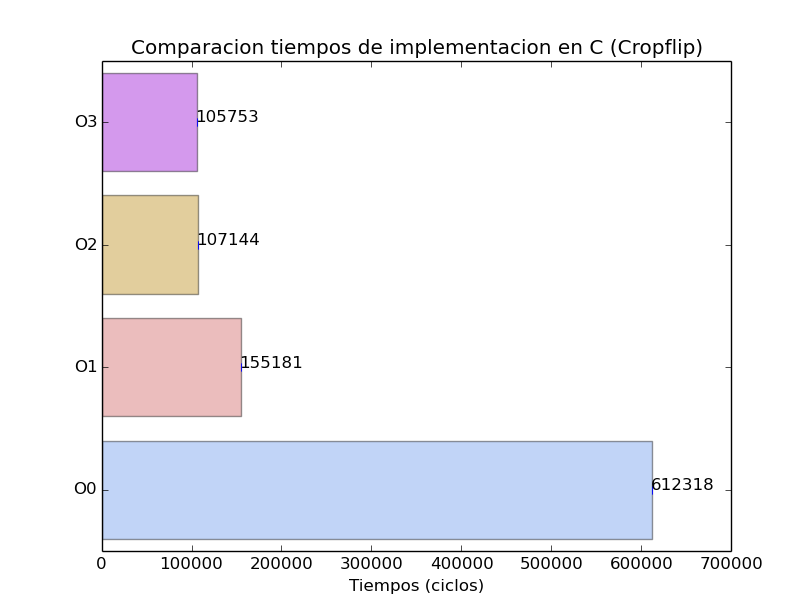
\includegraphics[width=350pt]{imagenes/cropCompC.png}

En el gr\'{a}fico se nota la clara diferencia entre las corridas con optimizaciones y sin ellas. El criterio fue el mismo que aplicamos en los experimentos de m\'{a}s adelante (Haciendo 1000 iteraciones).

\newpage

\textbf{Experimento 1.3)}\\ \\ 
En este experimento consideraremos diferentes criterios realizando siempre 10 mediciones, con outliers, sin ellos, y agregando programas en C++ que trabajen en simult\'{a}neo.\\ \\

\noindent \textbf{a)} \indent \textbf{Resultados:}\\ \\ 422861, 242136, 186857,\\ 194709, 234097, 221979,\\ 247912, 227976, 223245,\\ 200770.\\ \\ \\

\noindent\textbf{b)} \indent \textbf{Resultados:}\\ \\ 289209, 302654, 258757,\\ 254428, 248527, 254606,\\ 260391, 338981, 373612,\\ 280937 \\ \\ \\

\noindent \textbf{c)} \\ \textbf{10 mediciones}\\Esperanza: 240254.2 \\ Desv\'{i}o standard: 67250.78758 \\ Varianza: 4522668429.51111\\ \\
\noindent \textbf{10 mediciones con el programa en simult\'{a}neo:}\\Esperanza: 286210.2 \\ Desv\'{i}o standard: 41607.01932 \\
Varianza: 1731144056.62222\\ \\ \\
\textbf{d)} \textbf{10 mediciones sin 2 outliers:}\\Esperanza: 224103 \\ Desv\'{i}o standard: 18595.78063 \\ Varianza: 345803057.14286\\ \\ \\

\noindent \textbf{e)} \\
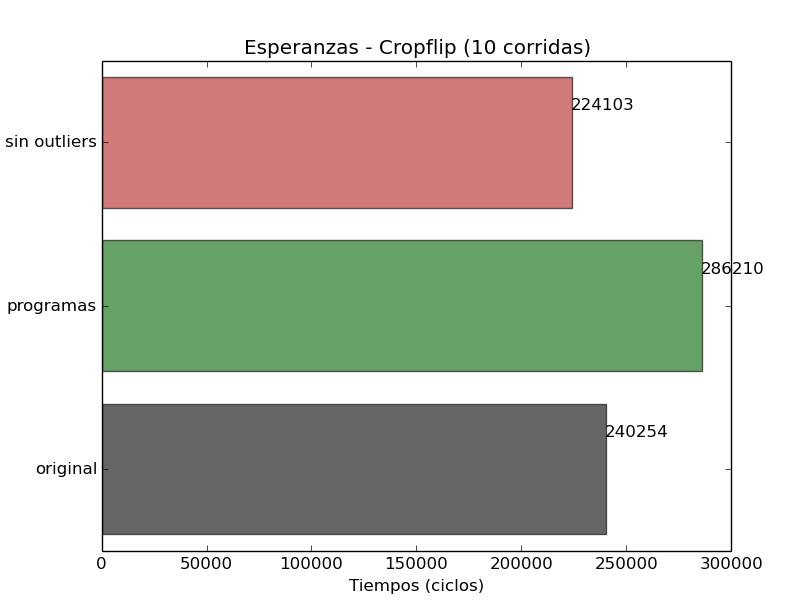
\includegraphics[width=300pt]{imagenes/esperanzas.png}

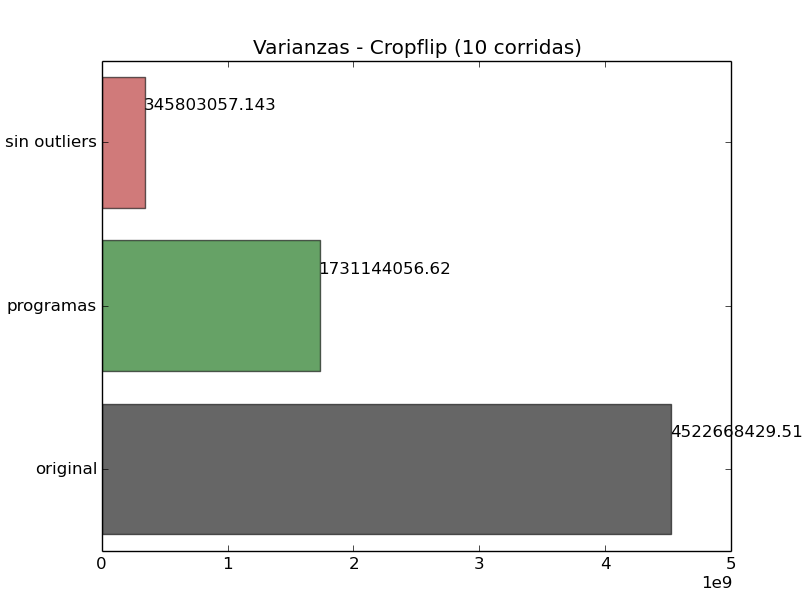
\includegraphics[width=300pt]{imagenes/varianzas.png}

Luego de observar estas mediciones hemos notado una varianza demasiado alta (y, en consecuencia, una falta de confiabilidad en las mediciones), por lo tanto, luego de probar con distintos m\'{e}todos de medici\'{o}n decidimos tomar el promedio de 1000 mediciones 10 veces, eliminar outliers y calcular luego nuevamente el promedio de las mediciones restantes.

\newpage

\textbf{Experimento 1.4)}\\ \\

Este experimento comparar\'{a} la performance de las implementaciones C y assembler que aplican el filtro cropflip (siguiendo el modelo de procesamiento secuencial y vectorial, respectivamente), probamos la implementaci\'{o}n en C con 4 distintos flags de optimizaci\'{o}n.

\begin{itemize}

\item \textbf{asm-} 46671 ciclos\\
\item \textbf{C O3-} 106740 ciclos\\
\item \textbf{C O2-} 106859 ciclos\\
\item \textbf{C O1-} 156148 ciclos\\
\item \textbf{C O0-} 613445 ciclos\\ \\ \\

\end{itemize}



NOTA: las l\'{i}neas peque\~nas azules en el tope de las barras representan el desv\'{i}o est\'{a}ndar del promedio de las mediciones que estamos mostrando.

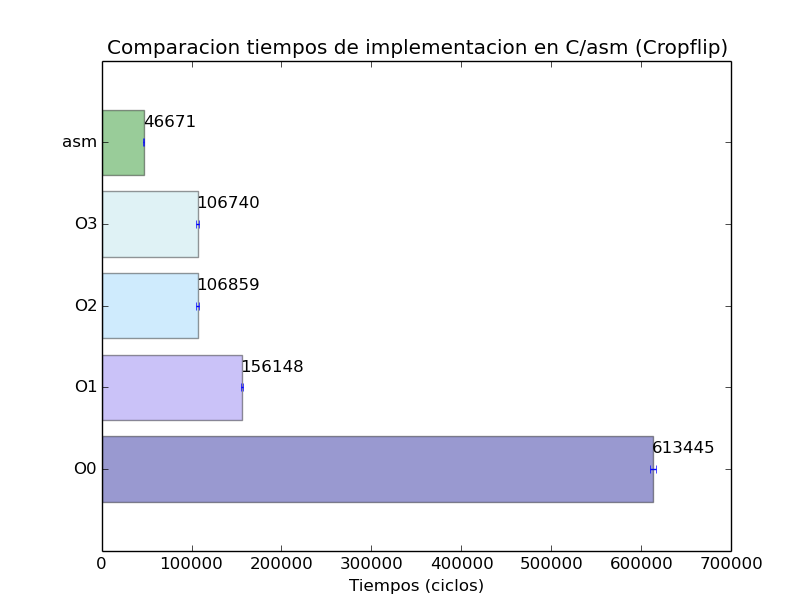
\includegraphics[width=300pt]{imagenes/CompCasm1.png}

Se observa en este experimento una notoria ventaja (en eficiencia temporal) del procesamiento vectorial de datos sobre el secuencial, incluso luego de haber aplicado las optimizaciones sobre el secuencial (que redujeron mucho el tiempo de procesamiento) la implementaci\'{o}n de assembler pudo aplicar el filtro mucho m\'{a}s r\'{a}pido y de manera m\'{a}s efectiva, mientras que entre las optimizaciones O2-O3 no hubo diferencia casi, indicando que no parece ser posible optimizar mucho m\'{a}s la implementaci\'{o}n en C.\\ \\ \\ \\

\newpage

\textbf{Experimento 1.5) Cropflip - cpu vs bus de memoria}\\ \\

blablalbla pregrafico
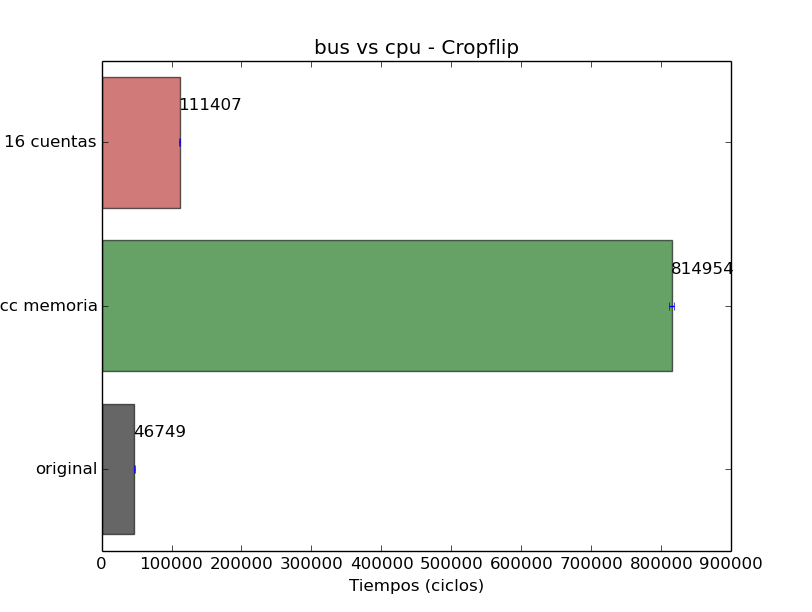
\includegraphics[width=300pt]{imagenes/bvmcrop.png}
blablabla postgrafico \\ \\ \\ \\

\subsubsection{Sierpinski}

\textbf{Experimento 2.1) Sierpinski - secuencial vs vectorial}\\ \\

Este experimento comparar\'{a} la performance de las implementaciones C y assembler que aplican el filtro sierpinski (siguiendo el modelo de procesamiento secuencial y vectorial, respectivamente), probamos la implementaci\'{o}n en C con 4 distintos flags de optimizaci\'{o}n.

\begin{itemize}


\item \textbf{asm-} 1618682 ciclos\\
\item \textbf{C O3-} 4114385  ciclos\\
\item \textbf{C O2-} 10599598 ciclos\\
\item \textbf{C O1-} 17026398 ciclos\\
\item \textbf{C O0-} 24125694 ciclos\\ \\ \\

\end{itemize}

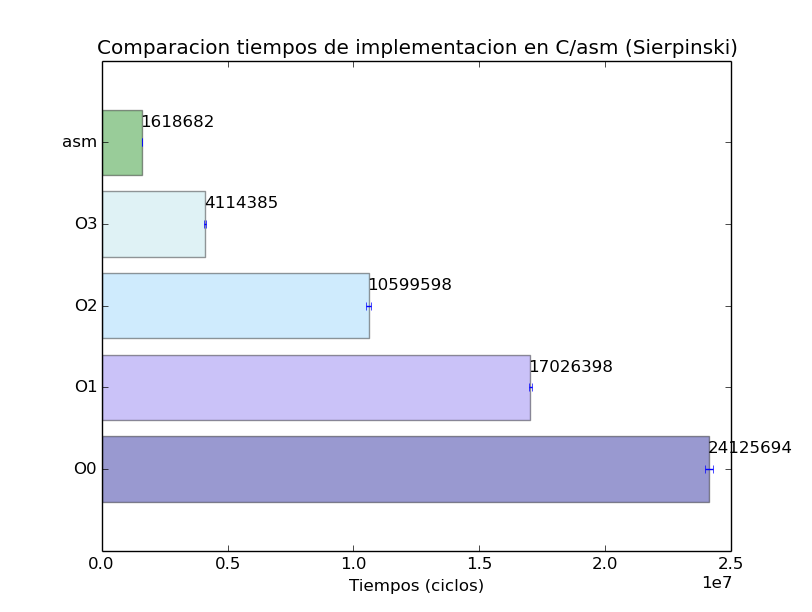
\includegraphics[width=350pt]{imagenes/CompCasm2.png}

En este experimento la ventaja de usar SIMD sigui\'{o} not\'{a}ndose con fuerza, mostrando una gran diferencia cuando es contrastado su tiempo de ejecuci\'{o}n con el de las distintas optimizaciones de la implementaci\'{o}n en C, si bien en este caso se not\'{o} que la optimizaci\'{o}n O3 tiene un gran impacto comparada con la O2. \\ \\ \\ \\

\textbf{Experimento 2.1) Sierpinski - cpu vs bus de memoria}\\ \\

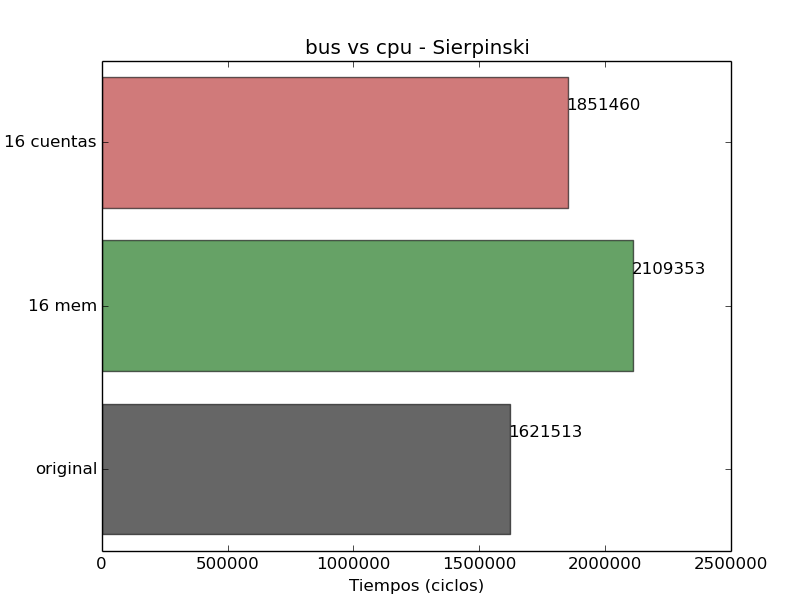
\includegraphics[width=300pt]{imagenes/bvmsierp.png}

\newpage

\subsubsection{Bandas}

\textbf{Experimento 3.1) Bandas - saltos condicionales}

En este experimento corrimos el programa con el flag -O1, en comparaci\'{o}n con el mismo programa sin los condicionales. Como explicamos en el punto 1.2, -O1 ofrece ciertas optimizaciones del c\'{o}digo que reducen sustancialmente el 'branching', reemplaz\'{a}ndolo en lo posible por instrucciones aritm\'{e}ticas. Por ello, ya esper\'{a}bamos cierta diferencia a favor del programa sin condicionales. Sin embargo al correr los experimentos nos sorprendi\'{o} que la diferencia era abismal: El c\'{o}digo sin condicionales corre 3 veces m\'{a}s r\'{a}pido que el optimizado. Esto deja en evidencia lo ineficiente que es utilizar saltos condicionales, incluso si lo optimizamos.

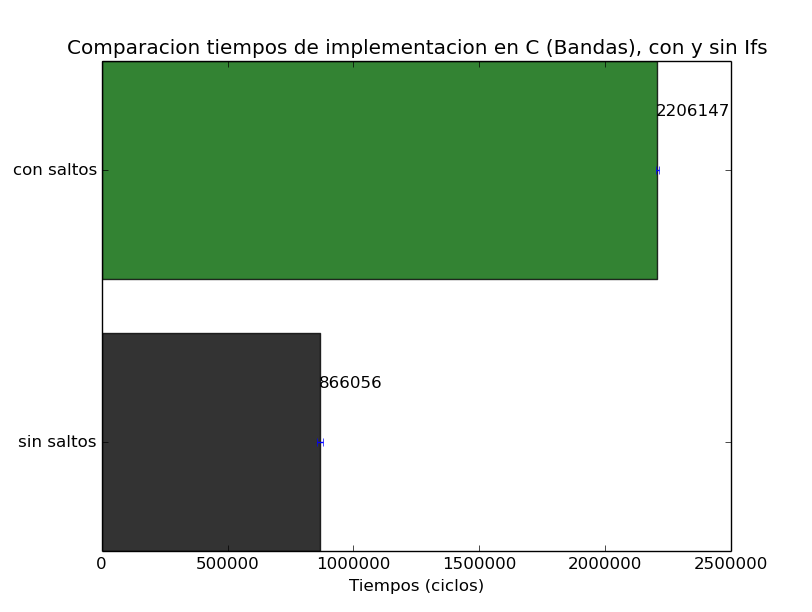
\includegraphics[width=350pt]{imagenes/cmpIFS.png}

\newpage

\textbf{Experimento 3.2) Bandas - secuencial vs vectorial}\\ \\

Este experimento comparar\'{a} la performance de las implementaciones C y assembler que aplican el filtro bandas (siguiendo el modelo de procesamiento secuencial y vectorial, respectivamente), probamos la implementaci\'{o}n en C con 4 distintos flags de optimizaci\'{o}n.

\begin{itemize}

\item \textbf{asm-}  516916 ciclos\\
\item \textbf{C O3-} 2205562 ciclos\\
\item \textbf{C O2-} 2165530 ciclos\\
\item \textbf{C O1-} 2214220 ciclos\\
\item \textbf{C O0-} 6931576 ciclos\\ \\ \\

\end{itemize}

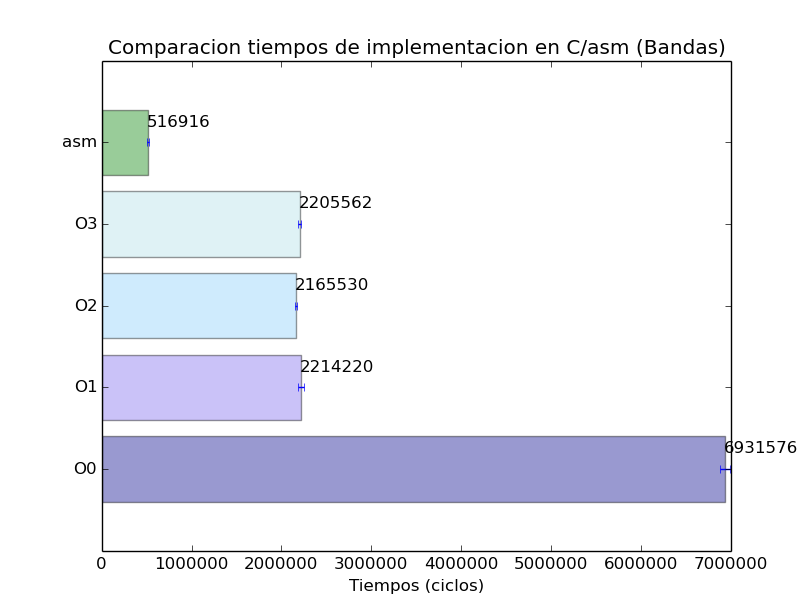
\includegraphics[width=350pt]{imagenes/CompCasm3.png}

\newpage

\subsubsection{Motion Blur}

\textbf{Experimento 4.1) Motion Blur - secuencial vs vectorial}\\ \\

Este experimento comparar\'{a} la performance de las implementaciones C y assembler que aplican el filtro motion blur (siguiendo el modelo de procesamiento secuencial y vectorial, respectivamente), probamos la implementaci\'{o}n en C con 4 distintos flags de optimizaci\'{o}n.

\begin{itemize}

\item \textbf{asm-}  1577304 ciclos
\item \textbf{C O3-} 4698057 ciclos\\
\item \textbf{C O2-} 4889967 ciclos\\
\item \textbf{C O1-} 5513945 ciclos\\
\item \textbf{C O0-} 17694922 ciclos\\\\ \\ \\

\end{itemize}

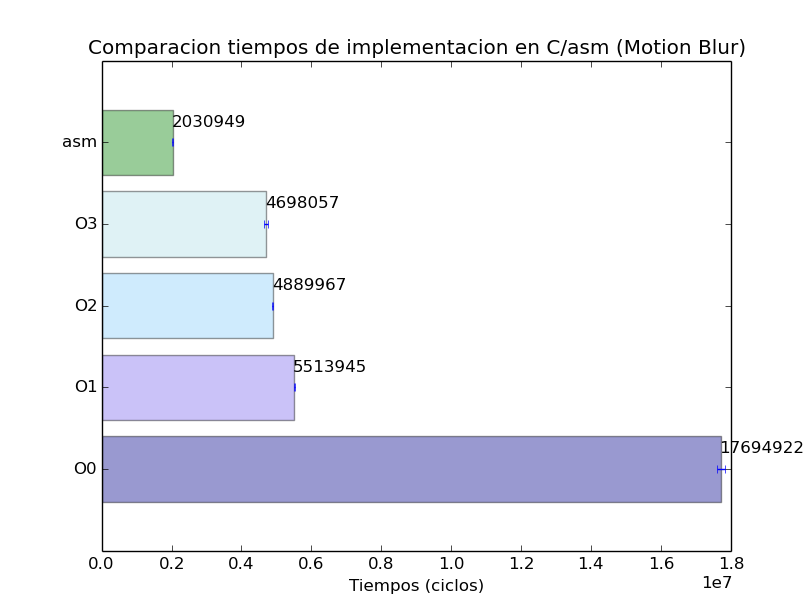
\includegraphics[width=350pt]{imagenes/CompCasm4.png}

En este experimento, nuevamente, la implementaci\'{o}n de assembler mostr\'{o} una clara diferencia (positiva) con las distintas optimizaciones de la de C, mientras que en C no se pudo optimizar el c\'{o}digo mucho m\'{a}s all\'{a} de la primera optimizaci\'{o}n.

\newpage

%\section{Enunciado y solucion} 
%\subsection{Filtro cropflip}

Programar el filtro \textit{cropflip} en lenguaje C y luego en ASM haciendo 
uso de las instrucciones vectoriales (\textbf{SSE}).

% ******************************************************************************
\vspace*{0.3cm} \noindent
\textbf{Experimento 1.1 - análisis el código generado}

En este experimento vamos a utilizar la herramienta \verb|objdump| para 
verificar como el compilador de C deja ensamblado el código C.

Ejecutar 
\begin{codesnippet}
\begin{verbatim}
objdump -Mintel -D cropflip_c.o
\end{verbatim}
\end{codesnippet}

¿Cómo es el código generado? 
Indicar
\begin{inparaenum}[\itshape a\upshape)]
    \item Por qué cree que hay otras funciones además de \verb|cropflip_c|
    \item Cómo se manipulan las variables locales
    \item Si le parece que ese código generado podría optimizarse
\end{inparaenum}

% ******************************************************************************
%\newpage
\vspace*{0.3cm} \noindent
\textbf{Experimento 1.2 - optimizaciones del compilador}

Compile el código de C con flags de optimización. Por ejemplo, pasando el flag 
\verb|-O1|\footnote{agregando este flag a \texttt{CCFLAGS64} en el makefile}. 
Indicar
\begin{inparaenum}
    \item Qué optimizaciones observa que realizó el compilador
    \item Qué otros flags de optimización brinda el compilador
    \item Los nombres de tres optimizaciones que realizan los compiladores.
\end{inparaenum}

% ------------------------------------------------------------------------------
% ------------------------------------------------------------------------------

\subsection{Mediciones}

Realizar una medición de performance \emph{rigurosa} es más difícil de lo 
que parece. 
En este experimento deberá realizar distintas mediciones de performance 
para verificar que sean buenas mediciones.

En un sistema ``ideal'' el proceso medido corre solo, sin ninguna 
interferencia de agentes externos. 
Sin embargo, una PC no es un sistema ideal. 
Nuestro proceso corre junto con decenas de otros, tanto de usuarios como 
del sistema operativo que compiten por el uso de la CPU. 
Esto implica que al realizar mediciones aparezcan ``ruidos'' o 
``interferencias'' que distorsionen los resultados.

El primer paso para tener una idea de si la medición es buena o no, 
es tomar varias muestras. 
Es decir, repetir la misma medición varias veces.
Luego de eso, es conveniente descartar los outliers
\footnote{en español, valor atípico: \url{http://es.wikipedia.org/wiki/Valor_atípico}}, 
que son los valores que más se alejan del promedio. 
Con los valores de las mediciones resultantes se puede calcular el promedio 
y también la varianza, que es algo similar el promedio de las distancias al 
promedio\footnote{en realidad, elevadas al cuadrado en vez de tomar el módulo}.

Las fórmulas para calcular el promedio $\mu$ y la varianza $\sigma^2$ son

$$
\mu = \frac{1}{n}\sum_{i=1}^{n} x_i \qquad \sigma^2 = \frac{\displaystyle\sum_{i=1}^{n}(x_i - \mu)^2} {n}
$$

% ******************************************************************************
\newpage
\vspace*{0.3cm} \noindent
\textbf{Experimento 1.3 - calidad de las mediciones}

\begin{enumerate}
    \item Medir el tiempo de ejecución de cropflip 10 veces. 
    \item Implementar un programa en C que no haga más que ciclar 
            infinitamente sumando 1 a una variable. 
            Lanzar este programa tantas veces como \emph{cores lógicos} tenga 
            su procesador. 
            Medir otras 10 veces mientras estos programas corren de fondo.
    \item Calcular el promedio y la varianza en ambos casos.
    \item Consideraremos outliers a los 2 mayores tiempos
     de ejecución de la medicion a) y también a los 2 menores,
     por lo que los descartaremos. Recalcular el promedio y la varianza después de hacer este descarte.
    \item Realizar un gráfico que presente estos dos últimos items.
\end{enumerate}

A partir de aquí todos los experimentos de mediciones deberán hacerse igual 
que en el presente ejercicio: tomando 10 mediciones, luego descartando 
outliers y finalmente calculando promedio y varianza.

% ******************************************************************************
%\newpage
\noindent\textbf{Experimento 1.4 - secuencial vs. vectorial}

En este experimento deberá realizar una medición de las diferencias de 
performance entre las versiones de C y ASM (el primero con -O0, -O1, -O2 y -O3) 
y graficar los resultados.

% ******************************************************************************
\vspace*{0.3cm} \noindent
\textbf{Experimento 1.5 - cpu vs. bus de memoria}

Se desea conocer cual es el mayor limitante a la
performance de este filtro en su versión ASM.

¿Cuál es el factor que limita la performance en este caso?
En caso de que el limitante fuera la intensidad de cómputo, entonces 
podrían agregarse instrucciones que realicen accesos a memoria extra y la
performance casi no debería sufrir. 
La inversa puede aplicarse, si el limitante es la cantidad de accesos a memoria.
\footnote{también podría pasar que estén más bien balanceados y que agregar
cualquier tipo de instrucción afecte sensiblemente la performance}
	
Realizar un experimento, agregando 4, 8 y 16 instrucciones aritméticas 
(por ej \verb|add rax, rbx|) analizando como varía el tiempo de ejecución.
Hacer lo mismo ahora con instrucciones de acceso a memoria, haciendo 
mitad lecturas y mitad escrituras (por ejemplo, agregando dos 
\verb|mov rax, [rsp]| y dos \verb|mov [rsp+8], rax|).\footnote{Notar que en el caso de acceder a \texttt{[rbp]} o \texttt{[rsp+8]} probablemente haya siempre hits en la cache, por lo que la medición no será de buena calidad. Si se le ocurre la manera, realizar accesos a otras direcciones alternativas.}
	
Realizar un único gráfico que compare:
\begin{inparaenum}
    \item La versión original
    \item Las versiones con más instrucciones aritméticas
    \item Las versiones com más accesos a memoria
\end{inparaenum}

Acompañar al gráfico con una tabla que indique los valores graficados.  
  
%\vspace*{0.3cm} \noindent
%\textbf{Experimento 1.6 (\textit{opcional}) - secuencial vs. vectorial (parte II)}
%
%
%Si vemos a los pixeles como una tira muy larga de
%bytes, este filtro en realidad no requiere \emph{casi}
%ningún procesamiento de datos en paralelo. Esto podría
%significar que la velocidad del filtro de C puede
%aumentarse hasta casi alcanzar la del de ASM. ¿ocurre esto?
%	
%Modificar el filtro para que en vez de acceder
%a los bytes de a uno a la vez se accedan como
%tiras de 64 bits y analizar la performance.

% ------------------------------------------------------------------------------
% ------------------------------------------------------------------------------

\subsection*{Filtro \textit{Sierpinski}}

Programar el filtro \textit{Sierpinski} en lenguaje C y en en ASM haciendo 
uso de las instrucciones vectoriales (\textbf{SSE}).

% ******************************************************************************
\vspace*{0.3cm} \noindent
\textbf{Experimento 2.1 - secuencial vs. vectorial}

Analizar cuales son las diferencias de performace entre las versiones de C 
y ASM de este filtro, de igual modo que para el experimento 1.4.

% ******************************************************************************
\vspace*{0.3cm} \noindent
\textbf{Experimento 2.1 - cpu vs. bus de memoria}

¿Cuál es el factor que limita la performance en este filtro?
Repetir el experimento 1.5 para este filtro.

\subsection*{Filtro \textit{Bandas}}

Programar el filtro \textit{Bandas} en lenguaje C y en en ASM haciendo uso de 
las instrucciones vectoriales (\textbf{SSE}).

% ******************************************************************************
\vspace*{0.3cm} \noindent
\textbf{Experimento 3.1 - saltos condicionales}

Se desea conocer que tanto impactan los saltos condicionales en el código 
de filtro Bandas con \verb|-O1| (la versión en C).\\
Para poder medir esto de manera aproximada, remover el código
que detecta a que banda pertenece cada pixel, dejando
sólo una banda.
Por más que la imagen resultante no sea correcta, será posible tomar una
medida aproximada del impacto de los saltos condicionales.
Analizar como varía la performance. 

% ******************************************************************************
\vspace*{0.3cm} \noindent
\textbf{Experimento 3.2 - secuencial vs. vectorial}

Repetir el experimento 1.4 para este filtro.

% ------------------------------------------------------------------------------
% ------------------------------------------------------------------------------

\subsection*{Filtro \textit{Motion Blur}}
Programar el filtro \textit{mblur} en lenguaje C y en ASM haciendo uso de 
las instrucciones \textbf{SSE}.

% ******************************************************************************
\vspace*{0.3cm} \noindent
\textbf{Experimento 4.1}

Repetir el experimento 1.4 para este filtro


\section{Conclusiones y trabajo futuro}


\end{document}

